\documentclass[11pt, a4paper]{article}
\usepackage{graphicx}
\usepackage{amsmath}
\usepackage{listings}
\usepackage{alltt}
\usepackage{url}
\usepackage[utf8]{inputenc}

\title{\bold{\underline{\textit{\Large{Assignment 4: Fourier Approximations}}}}}

\author{ROHIT KUMAR [EE20B111]}

\date{\today} 
\begin{document}	
		
\maketitle 
\section*{Abstract}
The main goals of this assignment are :-
\begin{itemize}
\item To fit two functions $e^{x}$ and $cos(cos(x))$ using their computed Fourier coefficients through direct integration.
\item To use least squares fitting method to compute the Fourier coefficients for the two functions $e^{x}$ and $cos(cos(x))$.
\item To understand and compare the variation in these two different methods by plotting graphs.
\end{itemize}


\section{Question 1}
{\textsl{\small{Define Python functions for the two functions above, that take a vector (or scalar) input, and return a vector (or scalar) value. Plot the functions over the interval [-2$\pi$,4$\pi$) in Figure 1 and 2 respectively.Determine whether the functions are periodic.  What function do you expect to be generated by the Fourier series? Compute and plot those functions as well in the respective figures.}}}

The following python code snippet is used to declare the functions $e^{x}$ and $cos(cos(x))$. Also, x \in [-2$\pi$ to 4$\pi$).

\begin{alltt}
def Exp(x):              
    return exp(x)       

def coscos(x):           
    return cos(cos(x))

x = linspace(-2*\pi, 4*\pi, 1200)
\end{alltt}

The below python code snippet is used to plot the graphs of $e^{x}$ and $cos(cos(x))$ function wrt to x:- 
\begin{verbatim}
    figure(1) 
    title("Semilog plot of $e^{x}$ function")
    xlabel(r'$x\rightarrow$', size = 15)
    ylabel(r'$e^x\rightarrow$', size = 15)	
    semilogy(x, Exp(x), 'r', label = 'True Value')	
    semilogy(x, Exp(t), '-b', label = 'Periodic Extension')	
    semilogy(xt, Est_C_Exp, 'go', label = 'Estimated Value') 
    grid(True) 
    legend() 
    show()

\end{verbatim}
The plots of $e^{x}$ and $cos(cos(x))$ are as shown below:-
   \begin{figure}[!tbh]
   	\centering
   	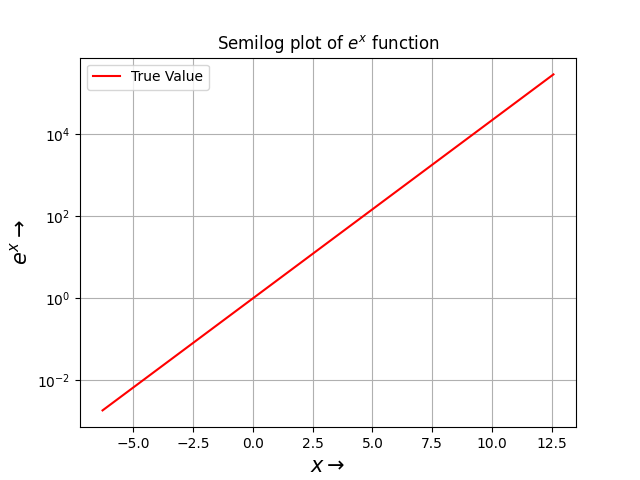
\includegraphics[scale=0.5]{Ass4_Figure_1.png}   
   	\caption{Semilog plot of $e^x$}
   	\label{fig:sample}
   \end{figure}



   
   \begin{figure}[!h]
   	\centering
   	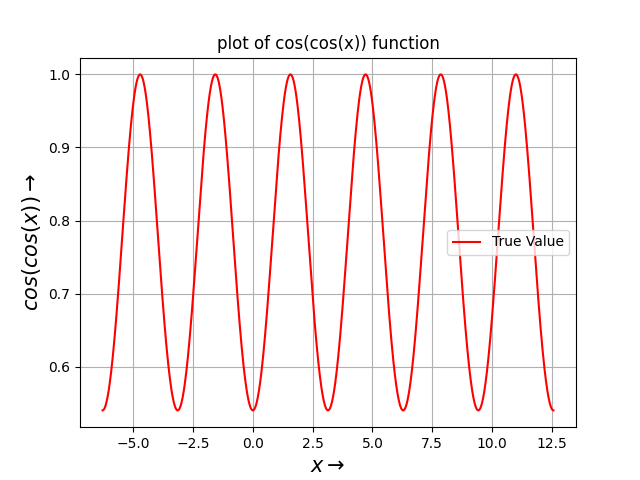
\includegraphics[scale=0.5]{Ass4_Figure_1.1.png}   
   	\caption{Plot of $cos(cos(x))$}
   	\label{fig:sample}
   \end{figure} 
   
\begin{verbatim}

    figure(2) 
    title("plot of cos(cos(x)) function") 
    xlabel(r'$x\rightarrow$',size = 15)	
    ylabel(r'$cos(cos(x))\rightarrow$',size = 15)
    plot(x, coscos(x),'r',label = 'True Value')	
    plot(x, coscos(t),'-b',label = 'Periodic Extension') 
    plot(xt, Est_C_coscos, 'go', label = 'Estimated Value')	
    grid(True)  
    legend() 
    show()
\end{verbatim}   
   
From the plots,It is evident that $e^{x}$ is aperiodic whereas $cos(cos(x))$ is periodic. The function $e^x$ is ever increasing with x and is non - periodic.The functions generated by the fourier series should be a periodic extension of  the actual functions. However for the evaluation of fourier series, the function is made 2$\pi$ periodic. The plots showing the periodic extensions of $e^{x}$ and $cos(cos(x))$ are as shown below along with actual functions :-

    \begin{figure}[!tbh]
   	\centering
   	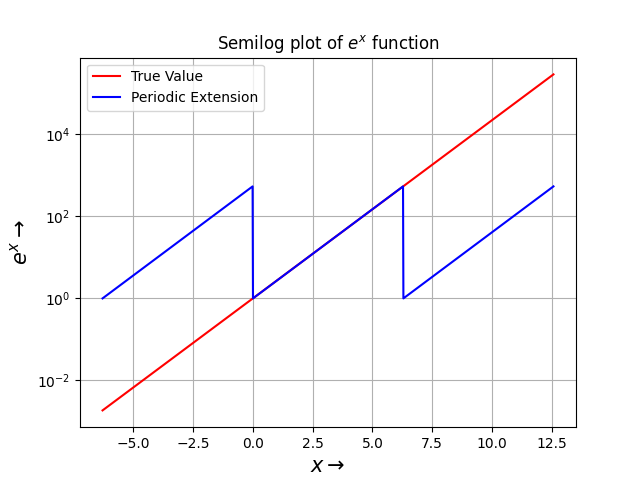
\includegraphics[scale=0.5]{Ass4_Figure_2.png}   
   	\caption{semilog plot for $e^x$}
   	\label{fig:sample}
   \end{figure} 
   
   \begin{figure}[!tbh]
   	\centering
   	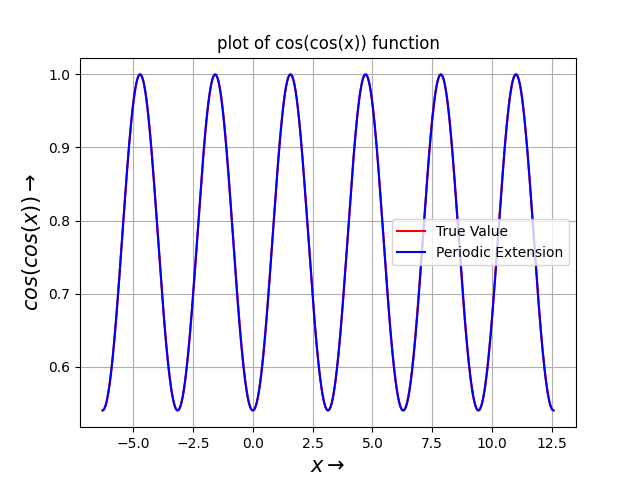
\includegraphics[scale=0.5]{Ass4_Figure_2.1.png}   
   	\caption{plot of $cos(cos(x))$}
   	\label{fig:sample}
   \end{figure}
   
\section{Question 2 and 3}
\subsection*{\textsl{\small{Obtain the first 51 coefficients for the two functions above by using quad function by applying the limits.Create a matrix of size 51*1 with the coefficients.For each of the two functions, make two different plots using “semilogy” and “loglog” and plot the magnitude of the coefficients vs n.}}}

\paragraph{To define the python functions the actual function and equations are as follows:-}

\begin{equation}
    a_{0} + \sum\limits_{n=1}^{\infty} {{a_{n}\cos(nx_{i})+b_{n}\sin(nx_{i})}} \approx f(x_{i}) 
    \end{equation}
    	The equations used here to find the Fourier coefficients are as follows:
    \begin{equation}
         a_{0} = \frac{1}{2\pi}\int\limits_{0}^{2\pi} f(x)dx  
    \end{equation}
    \begin{equation}
         a_{n} = \frac{1}{\pi}\int\limits_{0}^{2\pi} f(x)\cos(nx)dx 
    \end{equation}
    \begin{equation}
         b_{n} = \frac{1}{\pi}\int\limits_{0}^{2\pi} f(x)\sin(nx)dx 
    \end{equation}
First we are defining functions which are the inegrands that are present in formula to calculate fourier coefficients. Then the fourier coefficients are calculated using the quad function. We will use the \textit{quad()} function to perform an integration operation. Then we are assigning the values to a matrix with the 51 coefficients for both functions. The python code for finding the functions, finding the fourier coefficients and finding matrix is shown below. 
\begin{alltt}

def u_Exp(x, k):              
    return Exp(x) * cos(k*x)  

def v_Exp(x, k):              
    return Exp(x) * sin(k*x)  

def u_coscos(x, k):             
    return coscos(x) * cos(k*x) 

def v_coscos(x, k):             
    return coscos(x) * sin(k*x) 
	
xt = linspace(0, 2*\pi, 400) 
t = tile(xt, 3)
x = linspace(-2*\pi, 4*\pi, 1200)	

C_Exp = np.zeros((51, 1))	
C_Exp[0][0] = (1/(2*\pi))*(integrate.quad(Exp, 0, 2*\pi))[0] 	
for i in range(1, 26):	
	C_Exp[(2*i)-1][0] = (1/\pi)*(integrate.quad(u_Exp, 0, 2*\pi, args=(i)))[0]  
	C_Exp[2*i][0] = (1/\pi)*(integrate.quad(v_Exp, 0, 2*\pi, args=(i)))[0]

C_coscos = np.zeros((51,1))							
C_coscos[0][0] = (1/(2*\pi))*(integrate.quad(coscos, 0, 2*\pi))[0] 
for i in range(1,26):																	
	C_coscos[(2*i)-1][0] = (1/\pi)*(integrate.quad(u_coscos, 0, 2*\pi, args=(i)))[0]	
	C_coscos[2*i][0] = (1/\pi)*(integrate.quad(v_coscos, 0, 2*\pi, args=(i)))[0]
\end{alltt}

   
\subsection*{Plots of Fourier coefficients for both functions }
The semilog plot for the Magnitude of Fourier coefficients of  $e^{x}$ and the loglog plot for the Magnitude of fourier coefficients of $cos(cos(x))$ are shwn below:-
	\begin{figure}[!tbh]
   	\centering
   	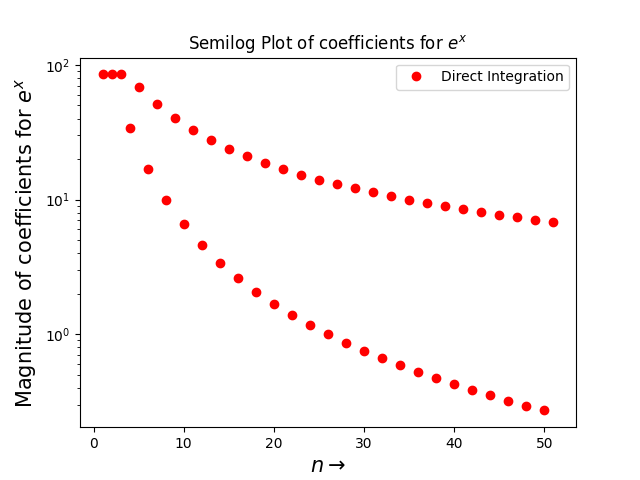
\includegraphics[scale=0.5]{Ass4_Figure_3.png}   
   	\caption{Semilog plot of the fourier coefficients of $e^{x}$}
   	\label{fig:sample}
   \end{figure} 

	\begin{figure}[!tbh]
   	\centering
   	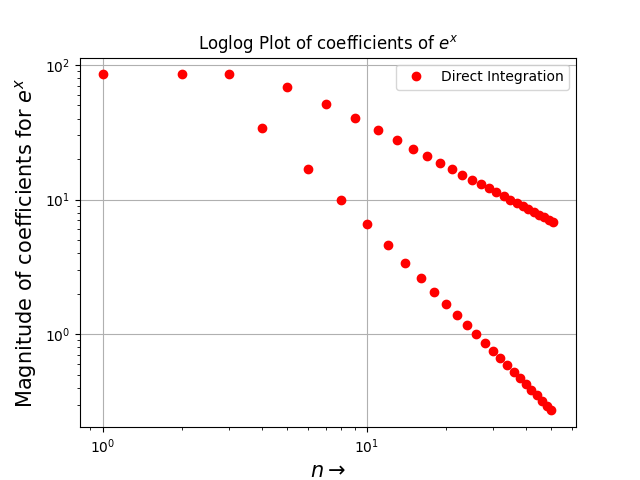
\includegraphics[scale=0.5]{Ass4_Figure_4.png}   
   	\caption{Loglog plot of the fourier coefficients of $e^{x}$}
   	\label{fig:sample}
   \end{figure} 
   \cleardoublepage
   
	\begin{figure}[!tbh]
   	\centering
   	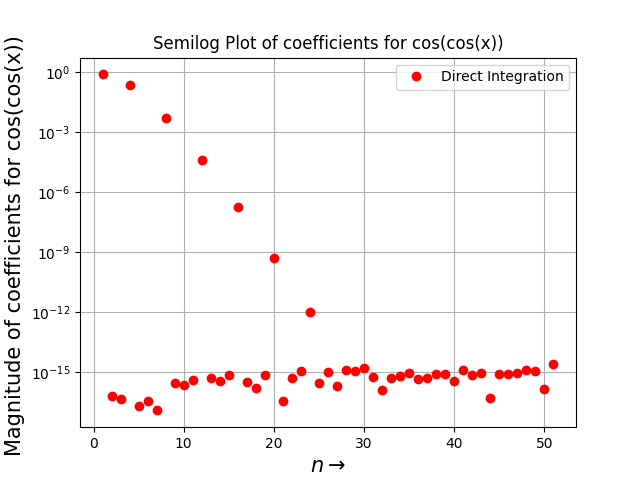
\includegraphics[scale=0.5]{Ass4_Figure_5.png}   
   	\caption{Semilog plot of the fourier coefficients of $cos(cos(x))$}
   	\label{fig:sample}
   \end{figure} 

	\begin{figure}[!tbh]
   	\centering
   	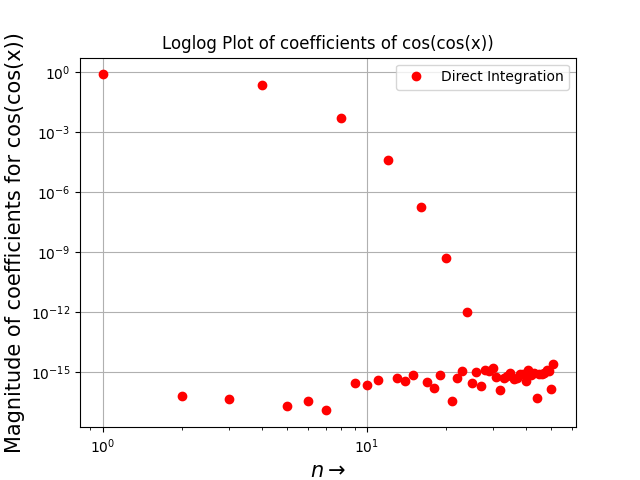
\includegraphics[scale=0.5]{Ass4_Figure_6.png}   
   	\caption{Loglog plot of the fourier coefficients of $cos(cos(x))$}
   	\label{fig:sample}
   \end{figure} 
1. From the plots, it is evident that $b_n$ coefficients are nearly zero for $cos(cos(x))$. Since $cos(cos(x))$ is an even function, it does not contain odd harmonics(the integrand becomes odd and hence whole integral is zero). Hence in the fourier series expansion, all the $b_n$ terms should be zero for the series to be an even function.\\\\
2. The magnitude of the coefficients would represent how much of certain frequencies happen to be in the output. $cos(cos(t))$ does not have very many frequencies of harmonics, so it dies out quickly. However, since the periodic extension of $e^{t}$ is discontinuous. To represent this discontinuity as a sum of continuous sinusoids, we would need high frequency components, hence coefficients do not decay as quickly.\\\\
3. The loglog plot looks linear for $e^{t}$ since Fourier coefficients of $e^{t}$ decay as a power of n, in particular, $a_n$ decays as $1/n$ and $b_n$ decays as $1/n^{2}$. The magnitude of the complex fourier coefficients of $e^x$ therefore decays as $1/n$. This is because of the discontinuities in the periodic extension of $e^x$. The semilog plot seems linear in the $cos(cos(t))$ case as its fourier coefficients decay exponentially with n.

\section{Question 4,5 and 6}
\subsection*{\textsl{Using least squares approach,Find the fouriers coefficients for both the functions by creating the matrix A, $A*c=b$.Plot the curves. Compare the answers got by least squares and by the direct integration.  }}
The fourier coefficients are estimated using least square estimation other than integration. For the least squares approach, we'll have to create matrices and then use \textit{lstsq()} function inorder to get the most approximate values of the fourier coefficients.\\
The python code  to create the matrices and to get the least squared value of the coefficients is as follows:

\begin{alltt}	
A = np.zeros((400, 51)) 
A[:, 0] = 1 
vector_x = linspace(0, 2*\pi, 401) 
vector_x = vector_x[:-1] 

for i in range(1, 26):
    A[:, 2*i-1] = cos(i*vector_x) 
    A[:, 2*i] = sin(i*vector_x) 
C_Expvector_x = Exp(vector_x)
C_coscosvector_x = coscos(vector_x)

lstsq_C_Exp = lstsq(A, C_Expvector_x, rcond=None)[0]	 
lstsq_C_coscos = lstsq(A, C_coscosvector_x, rcond=None)[0]
\end{alltt}

The plots in order to show the differences between the actual and predicted values of the fourier coefficients are shown below:-
\cleardoublepage

	\begin{figure}[!tbh]
   	\centering
   	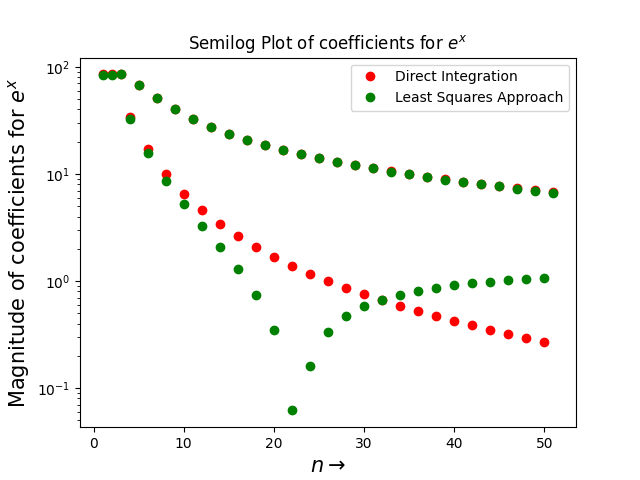
\includegraphics[scale=0.6]{Ass4_Figure_7.png}   
   	\caption{Semilog plots for $e^{x}$}
   	\label{fig:sample}
   \end{figure} 
   
   \begin{figure}[!tbh]
   	\centering
   	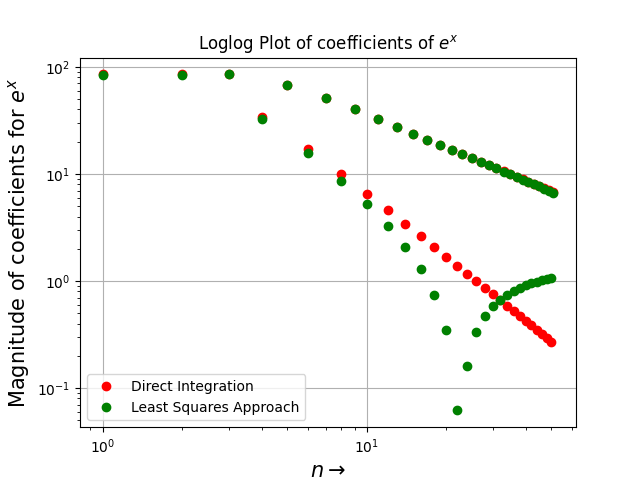
\includegraphics[scale=0.6]{Ass4_Figure_8.png}   
   	\caption{Loglog plots for $e^{x}$}
   	\label{fig:sample}
   \end{figure} 
   \begin{figure}[!tbh]
   	\centering
   	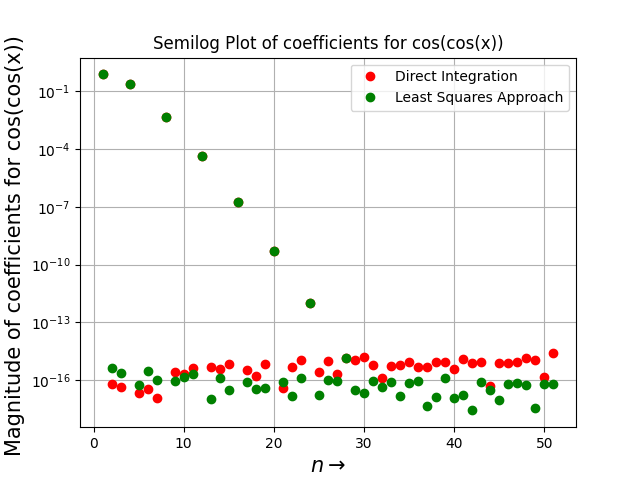
\includegraphics[scale=0.6]{Ass4_Figure_9.png}   
   	\caption{Semilog plots for $cos(cos(x))$}
   	\label{fig:sample}
   \end{figure} 
   
   \begin{figure}[!tbh]
   	\centering
   	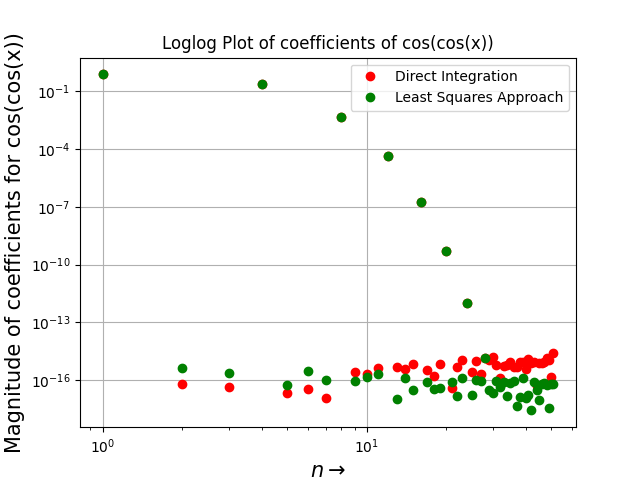
\includegraphics[scale=0.6]{Ass4_Figure_10.png}   
   	\caption{Loglog plots for $cos(cos(x))$}
   	\label{fig:sample}
   \end{figure} 
   \cleardoublepage
   
     

\section{Question 6} 
\subsection*{\textsl{Compare the answers got by least squares and by the direct integration. Do they agree? Should they?How much deviation is there (find the absolute difference between the two sets of coefficients and find the largest deviation. How will you do this using vectors?)}}
Since the least squares approach is only approximate method, slight deviation is expected from actual value.\\
The following python code used to calculate the absolute difference and largest deviation:-
\begin{verbatim}	
Abs_Diff_Exp = abs(lstsq_C_Exp - Ct_Exp)  
Abs_Diff_coscos = abs(lstsq_C_coscos - Ct_coscos)

Lar_Dev_Exp = max(Abs_Diff_Exp[0]) 
Lar_Dev_coscos = max(Abs_Diff_coscos[0])
\end{verbatim}
The largest deviation between coefficients for $e^{x}$ is 1.332730870335368\\
The largest deviation between coefficients for $cos(cos(x))$ is  2.669164544992301e-15\\\\
From the plots, the coefficients of $cos(cos(x))$ are more agreeable but not much agreeable for coefficients of $e^{x}$. This is because a significant deviation in $e^x$ case. The reason for this is $e^{x}$ function is not periodic and  $cos(cos(x))$ is periodic. The periodic extension of $e^{x}$ function is discontinuous and has increasing gradient. So, it require a more samples i.e $>>400$ to reduce the deviation and get accurate fourier coefficients. Even increasing the samples won't give exact result but helps to reduce the deviation mostly.The deviation is mostly seen at discontinues points.   


\section{Question 7}
\subsection*{\textsl{Compute Ac from the estimated values of c.  These should be the function values at xi. Plot them(with green circles) in Figures 1 and 2 respectively for the two functions.  Why is there so much deviation in Figure 1 but nearly perfect agreement in Figure 2?}}
Using the estimate values of the fourier coefficients, we can calculate the functional values for both $e^{x}$ and $cos(cos(x))$. \\
The matrix product $A*c=b$. By multiplication 400 functional values are obtained for both functions.\\
The python code for this matrix generation is as shown :-
\begin{verbatim}
Est_C_Exp = dot(A, lstsq_C_Exp) 
Est_C_coscos = dot(A, lstsq_C_coscos)
\end{verbatim}
The plots showing both the actual and estimated functional values are as shown below:

 	\begin{figure}[!tbh]
   	\centering
   	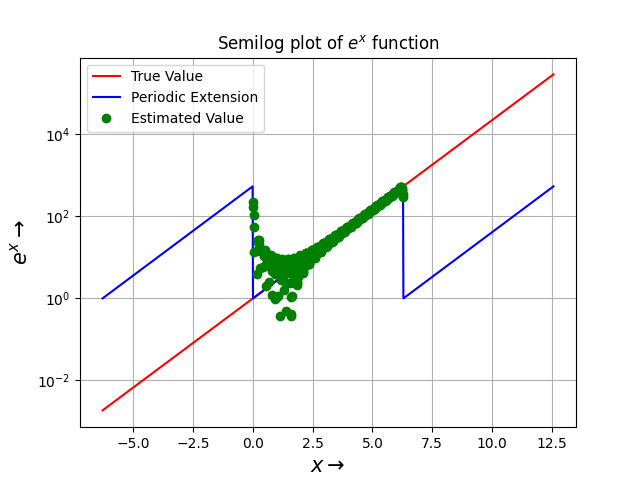
\includegraphics[scale=0.6]{Ass4_Figure_11.png}   
   	\caption{Actual and estimated values for $e^{x}$}
   	\label{fig:sample}
   \end{figure} 
   
   \begin{figure}[!tbh]
   	\centering
   	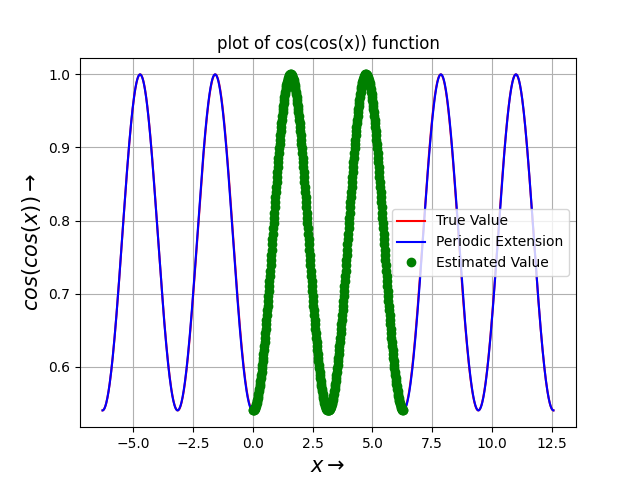
\includegraphics[scale=0.6]{Ass4_Figure_12.png}   
   	\caption{Actual and estimated values for $cos(cos(x))$}
   	\label{fig:sample}
   \end{figure}
   \cleardoublepage
   There is much deviation in Figure 1 but nearly perfect agreement in Figure 2 because it should be noted that Fourier series are for periodic functions. Without consideration the more samples in least square method, $cos(cos(x))$ plot is almost perfectly same. The reason why the $e^x$ plot is more deviated is the partial sums of the Fourier series will have large oscillations near the discontinuity of the function where n increases, these oscillations wont die out but reaches a finite limit. This is known Gibbs phenomenon.
	
\section*{Conclusions}
\begin{itemize}
\item The odd harmonics are zero for even functions in fourier coefficients calculation.The fourier series can be calculated by direct integration and also through least squares method.
\item The fourier series can be calculated by direct integration and also through least squares method.
\item More samples are to be taken to reduce the deviation in least squares. Mainly for discontinuous functions at discontinuous points.
\item For computation of fourirer coefficients, least squares method is not effective than direct integration in this case of fourier series(non-periodic).
\item The Gibbs phenomenon is observed at discontinuity points.
\end{itemize}

\end{document}